\documentclass[aspectratio=169,10pt]{beamer}

\usetheme{Madrid}
\usecolortheme{seahorse}

\usepackage{amsmath}
\usepackage{amssymb}
\usepackage{graphicx}
\usepackage{listings}
\usepackage{xcolor}
\usepackage{hyperref}
\usepackage{booktabs}

% Configure listings
\lstset{
    basicstyle=\ttfamily\scriptsize,
    commentstyle=\color{green!50!black}\itshape,
    keywordstyle=\color{blue}\bfseries,
    stringstyle=\color{red},
    numbers=left,
    numberstyle=\tiny\color{gray},
    frame=single,
    breaklines=true,
    breakatwhitespace=true,
    showstringspaces=false
}

% Set graphics path
\graphicspath{{figures/}}

% Set footer
\setbeamertemplate{footline}[frame number]

% Title page
\title{Stronger Notions of Monotonicity}
\subtitle{Chapter 22 - Convex Analysis and Monotone Operator Theory}
\author{Lecture Slides}
\date{}

\begin{document}

\begin{frame}
    \titlepage
\end{frame}

\begin{frame}{Chapter Overview}
    \tableofcontents
\end{frame}

% ============================================================================
% Section 1: Para, Strict, Uniform, and Strong Monotonicity
% ============================================================================

\section{Para, Strict, Uniform, and Strong Monotonicity}

\begin{frame}{Key Monotonicity Concepts}
    \begin{itemize}
        \item \textbf{Basic Monotonicity:} An operator $A: \mathcal{H} \to 2^{\mathcal{H}}$ is monotone if
            $$\langle x - y | u - v \rangle \geq 0$$
            for all $(x,u), (y,v) \in \text{gra } A$.

        \item This chapter explores \emph{stronger} notions of monotonicity:
            \begin{enumerate}
                \item Paramonotone
                \item Strictly monotone
                \item Uniformly monotone
                \item Strongly monotone
                \item Cyclically monotone
            \end{enumerate}

        \item Each notion imposes additional structure and properties
        \item Fundamental for understanding optimization algorithms
    \end{itemize}
\end{frame}

\begin{frame}{Paramonotone Operators}
    \begin{definition}
        Let $K$ be a real Hilbert space and let $A: \mathcal{H} \to 2^{\mathcal{H}}$ be an operator.
        Then $A$ is \textbf{paramonotone} if $A$ and $A^{-1}$ are both monotone.
    \end{definition}

    \begin{block}{Proposition 22.2}
        Let $K$ be a real Hilbert space, let $A: \mathcal{H} \to 2^{\mathcal{H}}$ and $B: \mathcal{K} \to 2^{\mathcal{K}}$ be
        paramonotone operators, and let $L \in \mathcal{B}(\mathcal{H}, \mathcal{K})$. Then:
        \begin{enumerate}
            \item[(i)] $A^{-1}$ is paramonotone
            \item[(ii)] $A + L^* B L$ is paramonotone
        \end{enumerate}
    \end{block}

    \vspace{0.5cm}
    \textbf{Intuition:} Both the operator and its inverse preserve the monotonicity structure.
\end{frame}

\begin{frame}{Strictly Monotone and Strictly Cocoercive Operators}
    \begin{definition}
        An operator $A$ is \textbf{strictly monotone} if $A$ is monotone and
        $$\langle x - y | u - v \rangle = 0, \quad (x,u), (y,v) \in \text{gra } A \implies x = y.$$
    \end{definition}

    \begin{definition}
        An operator $A$ is \textbf{strictly cocoercive} if there exists $\alpha \in ]0,1[$ such that
        $$\langle x - y | u - v \rangle \geq \alpha \|u - v\|^2.$$
    \end{definition}

    \vspace{0.5cm}
    \begin{example}[22.6]
        Let $D$ be a nonempty subset of $\mathcal{H}$, let $T: D \to \mathcal{H}$, let $\alpha \in [-1,1]$, and set $A = \text{Id} + \alpha T$.
        \begin{enumerate}
            \item[(i)] If $T$ is strictly nonexpansive, then $A$ is strictly monotone.
            \item[(ii)] If $T$ is $\beta$-Lipschitz continuous with $\beta \in [0,1]$, then $A$ is strongly monotone
                      with modulus $1 - |\alpha|\beta$.
        \end{enumerate}
    \end{example}
\end{frame}

\begin{frame}{Uniformly and Strongly Monotone Operators}
    \begin{definition}
        An operator $A$ is \textbf{uniformly monotone} with modulus $\phi: \mathbb{R}_+ \to [0, +\infty]$ if
        $$\langle x - y | u - v \rangle \geq \phi(\|x - y\|), \quad \forall (x,u), (y,v) \in \text{gra } A.$$
    \end{definition}

    \begin{definition}
        An operator $A$ is \textbf{strongly monotone} with constant $\beta \in \mathbb{R}_{++}$ if
        $$\langle x - y | u - v \rangle \geq \beta \|x - y\|^2, \quad \forall (x,u), (y,v) \in \text{gra } A.$$
    \end{definition}

    \vspace{0.5cm}
    \textbf{Hierarchy:}
    $$\text{Strongly Monotone} \implies \text{Uniformly Monotone} \implies \text{Monotone}$$
\end{frame}

\begin{frame}{Monotonicity of Subdifferentials}
    \begin{example}[22.4]
        Let $f: \mathcal{H} \to ]-\infty, +\infty]$ be proper and convex. Then:
        \begin{enumerate}
            \item[(i)] $\partial f$ is paramonotone.
            \item[(ii)] If $f$ is strictly convex, then $\partial f$ is strictly monotone.
            \item[(iii)] If $f$ is uniformly convex with modulus $\phi$, then $\partial f$ is uniformly monotone
                       with modulus $2\phi$.
            \item[(iv)] If $f$ is strongly convex with constant $\beta \in \mathbb{R}_{++}$, then $\partial f$ is
                       strongly monotone with constant $\beta$.
        \end{enumerate}
    \end{example}

    \vspace{0.5cm}
    \textbf{Key insight:} Monotonicity properties of $\partial f$ reflect the convexity structure of $f$.
\end{frame}

\begin{frame}{Existence and Uniqueness}
    \begin{example}[22.12]
        Let $A: \mathcal{H} \to \mathcal{H}$ be monotone and hemicontinuous, and let $r \in \mathcal{H}$.
        Suppose that one of the following holds:
        \begin{enumerate}
            \item[(i)] $A$ is strictly monotone and $\lim_{\|x\| \to +\infty} \|Ax\| = +\infty$.
            \item[(ii)] $A$ is uniformly monotone with a supercoercive modulus.
            \item[(iii)] $A$ is strongly monotone.
        \end{enumerate}

        Then the equation $Ax = r$ has \emph{exactly one solution}.
    \end{example}

    \vspace{0.5cm}
    \textbf{Importance:} Monotonicity directly implies solvability of linear systems with monotone operators.
\end{frame}

% ============================================================================
% Section 2: Cyclic Monotonicity
% ============================================================================

\section{Cyclic Monotonicity}

\begin{frame}{Definition of Cyclic Monotonicity}
    \begin{definition}[22.13]
        Let $A: \mathcal{H} \to 2^{\mathcal{H}}$ and let $n \in \mathbb{N}$ be such that $n \geq 2$.
        Then $A$ is \textbf{$n$-cyclically monotone} if, for every $(x_1, \ldots, x_{n+1}) \in \mathcal{H}^{n+1}$
        and every $(u_1, \ldots, u_n) \in \mathcal{H}^n$,

        $$\left.\begin{array}{l}
            (x_1, u_1) \in \text{gra } A, \\
            \vdots \\
            (x_n, u_n) \in \text{gra } A, \\
            x_{n+1} = x_1
        \end{array}\right\} \implies \sum_{i=1}^{n} \langle x_{i+1} - x_i | u_i \rangle \leq 0.$$
    \end{definition}

    \vspace{0.3cm}
    \begin{block}{Remark}
        \begin{itemize}
            \item If $A$ is $n$-cyclically monotone for every $n \geq 2$, then $A$ is \textbf{cyclically monotone}.
            \item \textbf{2-cyclic monotonicity} is ordinary monotonicity.
        \end{itemize}
    \end{block}
\end{frame}

\begin{frame}{Visual Example of Cyclic Monotonicity}
    \begin{center}
        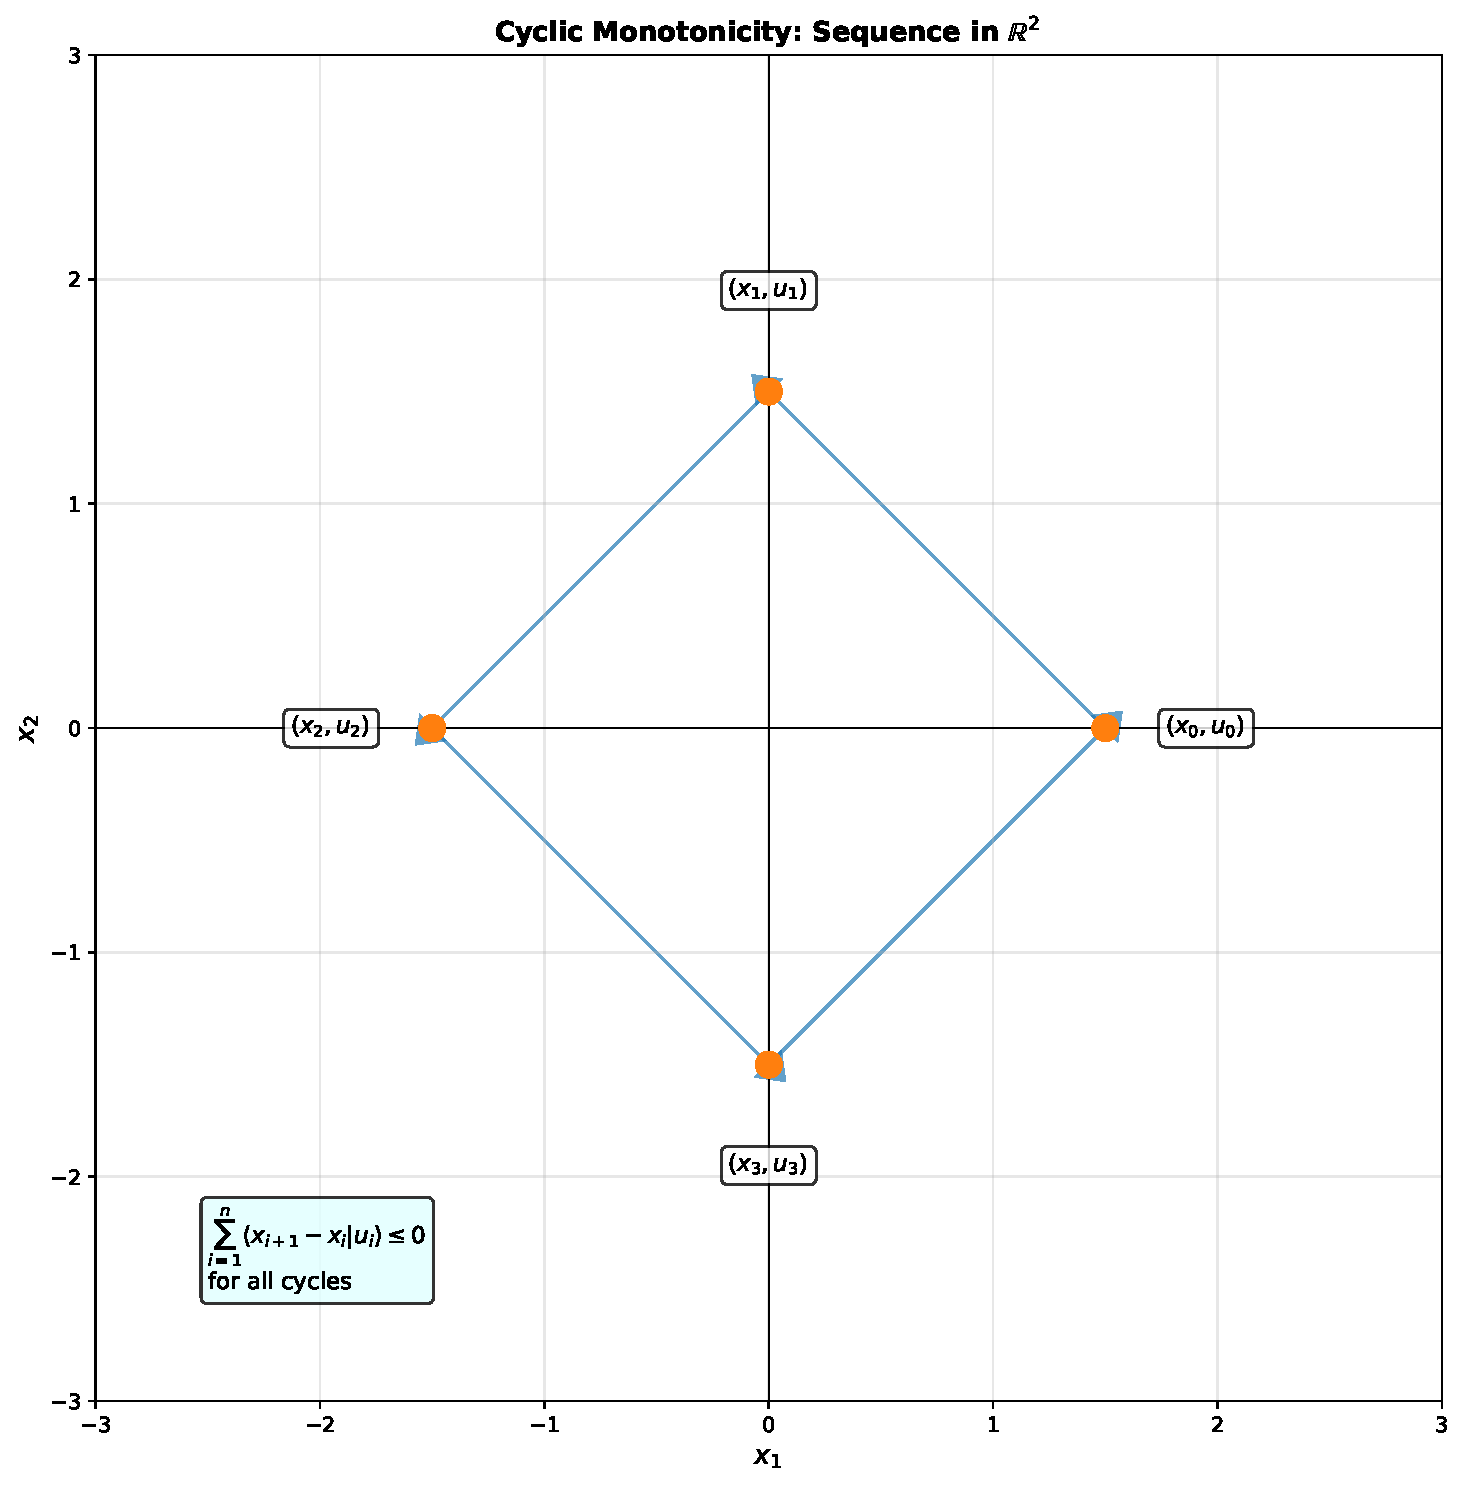
\includegraphics[width=0.8\textwidth]{fig_cyclic_sequence.pdf}
    \end{center}

    A cyclic sequence $(x_1, u_1), \ldots, (x_n, u_n)$ in the graph of $A$ satisfies:
    $$\sum_{i=1}^{n} \langle x_{i+1} - x_i | u_i \rangle \leq 0$$
    where indices are taken modulo $n$.
\end{frame}

\begin{frame}{Cyclic Monotonicity of Subdifferentials}
    \begin{block}{Proposition 22.14}
        Let $f: \mathcal{H} \to ]-\infty, +\infty]$ be proper. Then $\partial f$ is cyclically monotone.
    \end{block}

    \begin{proof}[Proof Sketch]
        Fix $n \geq 2$. For every $i \in \{1, \ldots, n\}$, take $(x_i, u_i) \in \text{gra } \partial f$.
        By property (16.1) of subdifferentials:
        $$\langle x_{i+1} - x_i | u_i \rangle \leq f(x_{i+1}) - f(x_i).$$

        Summing over the cycle and using $x_{n+1} = x_1$:
        $$\sum_{i=1}^{n} \langle x_{i+1} - x_i | u_i \rangle \leq \sum_{i=1}^{n} (f(x_{i+1}) - f(x_i)) = 0.$$
    \end{proof}
\end{frame}

\begin{frame}{Not All Maximal Monotone Operators are Cyclically Monotone}
    \begin{example}[22.15]
        Suppose $\mathcal{H} = \mathbb{R}^2$, and set
        $$A = \begin{bmatrix} 0 & -1 \\ 1 & 0 \end{bmatrix}.$$

        Then $A$ is maximally monotone but \textbf{not} 3-cyclically monotone.
    \end{example}

    \begin{block}{Remark}[22.16]
        The operator $A$ in Example 22.15 is a counterclockwise rotation by $\pi/2$.
        More generally, a counterclockwise rotation in $\mathbb{R}^2$ by angle $\theta \in [0, \pi/2[$
        is $n$-cyclically monotone if and only if $\theta \in [0, \pi/n]$.
    \end{block}

    \vspace{0.3cm}
    \textbf{Insight:} Cyclic monotonicity is a genuinely stronger condition than maximal monotonicity.
\end{frame}

\begin{frame}{Cyclic Monotonicity and Paramonotonicity}
    \begin{block}{Proposition 22.17}
        Let $A: \mathcal{H} \to 2^{\mathcal{H}}$ be 3-cyclically monotone and maximally monotone.
        Then $A$ is paramonotone.
    \end{block}

    \begin{proof}[Proof Sketch]
        For points $(x,u), (y,v) \in \text{gra } A$ with $\langle x - y | u - v \rangle = 0$:

        By 3-cyclic monotonicity, for any $(z, w) \in \text{gra } A$:
        $$0 \geq \langle y - x | u \rangle + \langle z - y | v \rangle + \langle x - z | w \rangle$$

        Using the zero inner product and monotonicity arguments, we can show that
        both $(x,u)$ and $(y,u)$ belong to $\text{gra } A$.
    \end{proof}
\end{frame}

% ============================================================================
% Section 3: Rockafellar's Cyclic Monotonicity Theorem
% ============================================================================

\section{Rockafellar's Cyclic Monotonicity Theorem}

\begin{frame}{The Fundamental Result}
    \begin{theorem}[22.18 - Rockafellar]
        Let $A: \mathcal{H} \to 2^{\mathcal{H}}$. Then $A$ is maximally cyclically monotone if and only if
        there exists $f \in \Gamma_0(\mathcal{H})$ such that $A = \partial f$.
    \end{theorem}

    \vspace{0.5cm}
    \textbf{Significance:}
    \begin{itemize}
        \item Establishes a \emph{complete characterization} of subdifferentials via cyclic monotonicity
        \item Every subdifferential is cyclically monotone (Proposition 22.14)
        \item Conversely, every maximally cyclically monotone operator arises as a subdifferential
        \item Bridges monotone operator theory and convex analysis
    \end{itemize}
\end{frame}

\begin{frame}{Rockafellar's Theorem - Key Construction}
    \begin{theorem}[22.18 - Rockafellar (continued)]
    \textbf{Proof Strategy (converse direction):} Given a maximally cyclically monotone operator $A$:

    \begin{enumerate}
        \item Define $f: \mathcal{H} \to [-\infty, +\infty]$ by
            $$f(x) := \sup_{n \geq 1} \sup_{(x_1, u_1), \ldots, (x_n, u_n) \in \text{gra } A}
            \left\{ \langle x - x_n | u_n \rangle + \sum_{i=0}^{n-1} \langle x_{i+1} - x_i | u_i \rangle \right\}$$

        \item Show that $f \in \Gamma_0(\mathcal{H})$ using cyclic monotonicity

        \item Prove that $\text{gra } A \subseteq \text{gra } \partial f$

        \item Use maximal cyclic monotonicity to conclude $A = \partial f$
    \end{enumerate}
    \end{theorem}

    \vspace{0.3cm}
    This is a deep result connecting graph properties to convex functions.
\end{frame}

\begin{frame}{Rockafellar's Theorem - Visual Summary}
    \begin{center}
        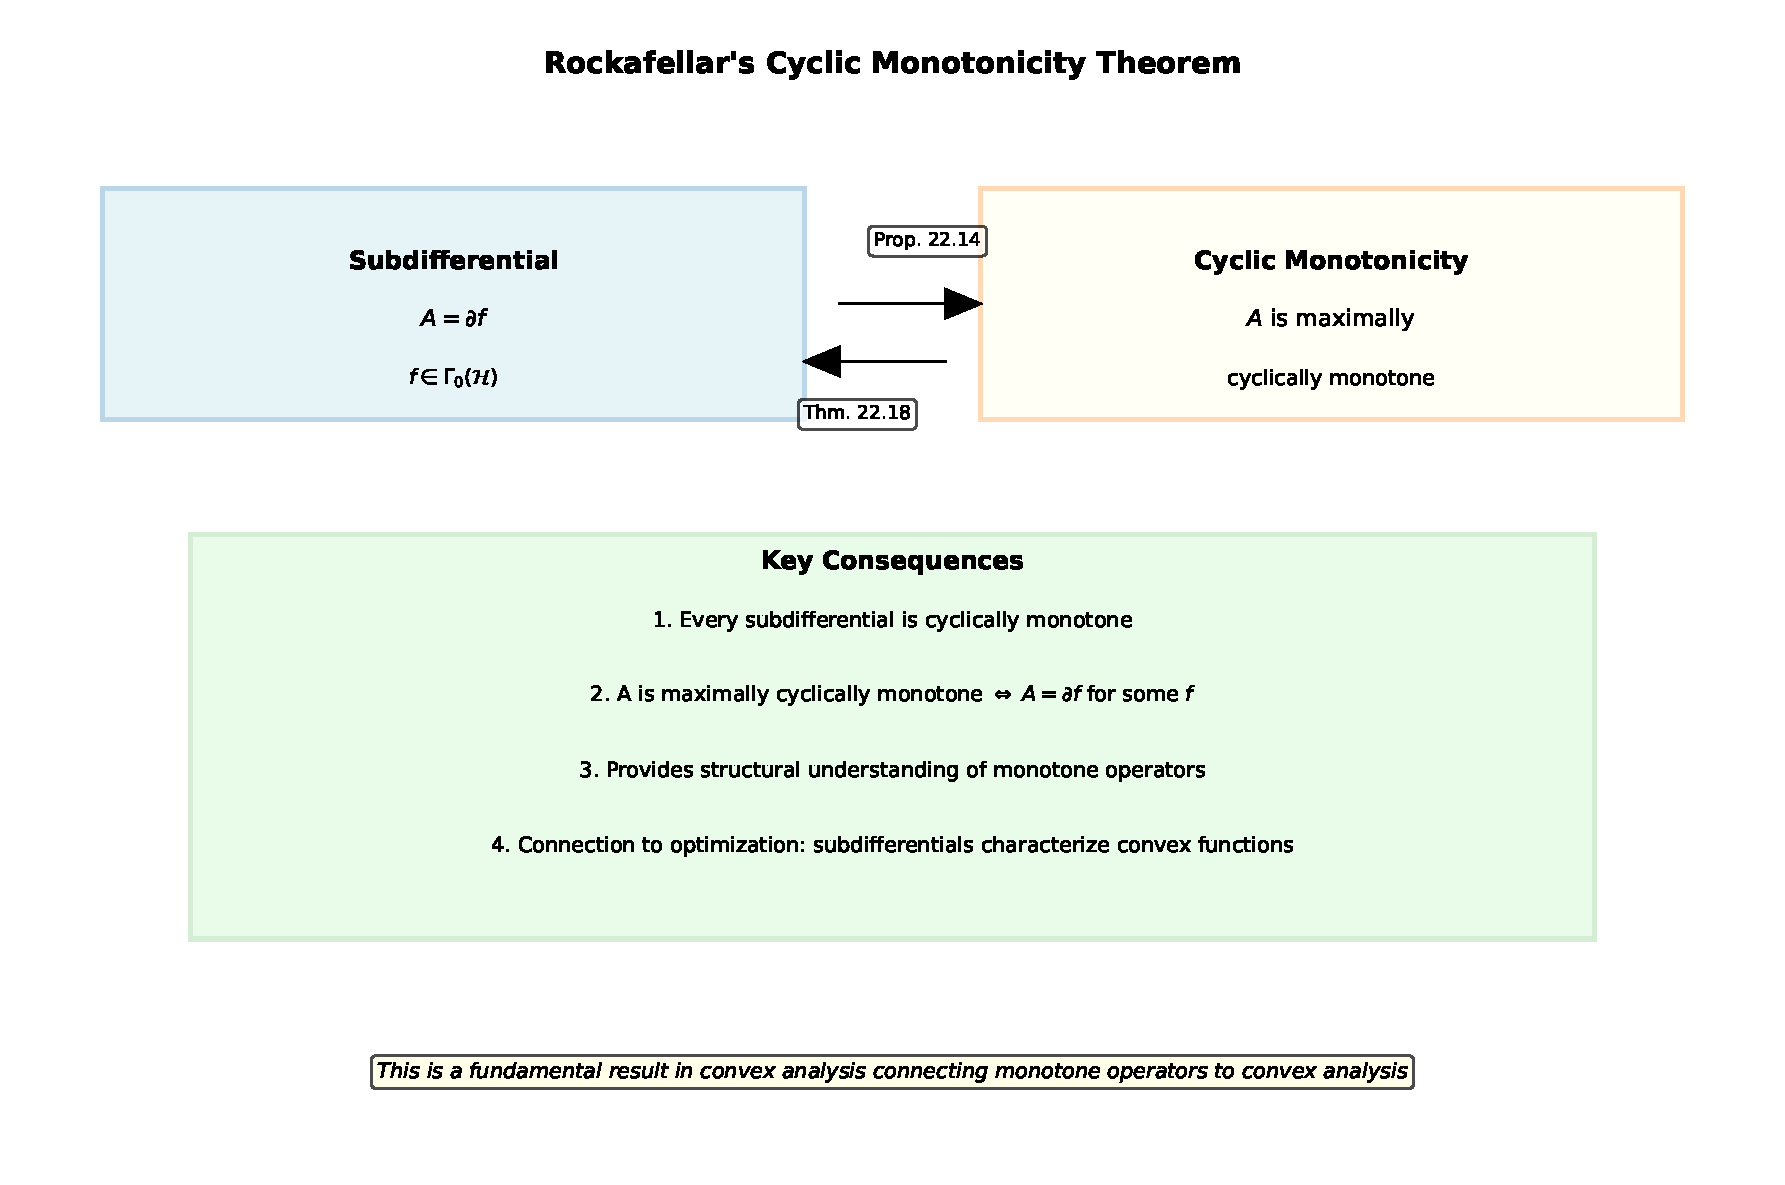
\includegraphics[width=\textwidth]{fig_rockafellar_theorem.pdf}
    \end{center}
\end{frame}

\begin{frame}{Uniqueness of Subdifferentials}
    \begin{block}{Proposition 22.19}
        Let $f$ and $g$ be functions in $\Gamma_0(\mathcal{H})$ such that $\partial f = \partial g$.
        Then there exists $\gamma \in \mathbb{R}$ such that $f = g + \gamma$.
    \end{block}

    \begin{proof}[Proof Idea]
        Consider the special case where $f$ and $g$ are differentiable.
        If $\partial f = \partial g$, then $\nabla f = \nabla g$ everywhere,
        which implies $f - g$ is constant.

        The general case follows by approximation techniques using
        $\square g$ and the conjugate operations.
    \end{proof}

    \vspace{0.3cm}
    \textbf{Consequence:} Subdifferentials determine convex functions up to an additive constant.
\end{frame}

% ============================================================================
% Section 4: Monotone Operators on ℝ
% ============================================================================

\section{Monotone Operators on $\mathbb{R}$}

\begin{frame}{Characterization on One Dimension}
    \begin{definition}
        We introduce a binary relation on $\mathbb{R}^2$ via
        $$\forall x_1 = (x_1, u_1) \in \mathbb{R}^2 ~ \forall x_2 = (x_2, u_2) \in \mathbb{R}^2:
        \quad x_1 \preceq x_2 \Leftrightarrow x_1 \leq x_2 \text{ and } u_1 \leq u_2.$$
        We write $x_1 \prec x_2$ if $x_1 \preceq x_2$ and $x_1 \neq x_2$.
    \end{definition}

    \begin{block}{Proposition 22.20}
        $(\mathbb{R}^2, \preceq)$ is directed and partially ordered, but \textbf{not} totally ordered.
    \end{block}

    \vspace{0.3cm}
    \textbf{Remark:} This partial order is crucial for analyzing monotone relations in $\mathbb{R}^2$.
\end{frame}

\begin{frame}{Main Equivalence in One Dimension}
    \begin{theorem}[22.22]
        Let $A: \mathbb{R} \to 2^{\mathbb{R}}$ be such that $\text{gra } A \neq \emptyset$.
        Then $A$ is monotone if and only if it is \textbf{cyclically monotone}.
    \end{theorem}

    \begin{corollary}[22.23]
        Let $A: \mathbb{R} \to 2^{\mathbb{R}}$ be maximally monotone. Then there exists
        $f \in \Gamma_0(\mathbb{R})$ such that $A = \partial f$.
    \end{corollary}

    \vspace{0.3cm}
    \textbf{Implication:} In $\mathbb{R}$, monotone and cyclically monotone are equivalent!
    Thus Rockafellar's theorem specializes nicely in one dimension.
\end{frame}

\begin{frame}{Intuition for One-Dimensional Case}
    In $\mathbb{R}$, the structure is particularly rigid:

    \begin{itemize}
        \item The partial order $\preceq$ on $\mathbb{R}^2$ has a special structure
        \item Any monotone chain in $\mathbb{R}^2$ is automatically cyclically monotone
        \item This is because we cannot have "loops" in the monotone relation when restricted to one dimension
        \item Consequently, every maximally monotone operator in $\mathbb{R}$ must arise as a subdifferential
    \end{itemize}

    \vspace{0.5cm}
    \begin{center}
        \textbf{Contrast:} In higher dimensions, we can have maximally monotone operators
        (like rotations) that are not cyclically monotone.
    \end{center}
\end{frame}

% ============================================================================
% Section 5: Summary and Relationships
% ============================================================================

\section{Summary and Relationships}

\begin{frame}{Comparison of Monotonicity Types}
    \begin{center}
        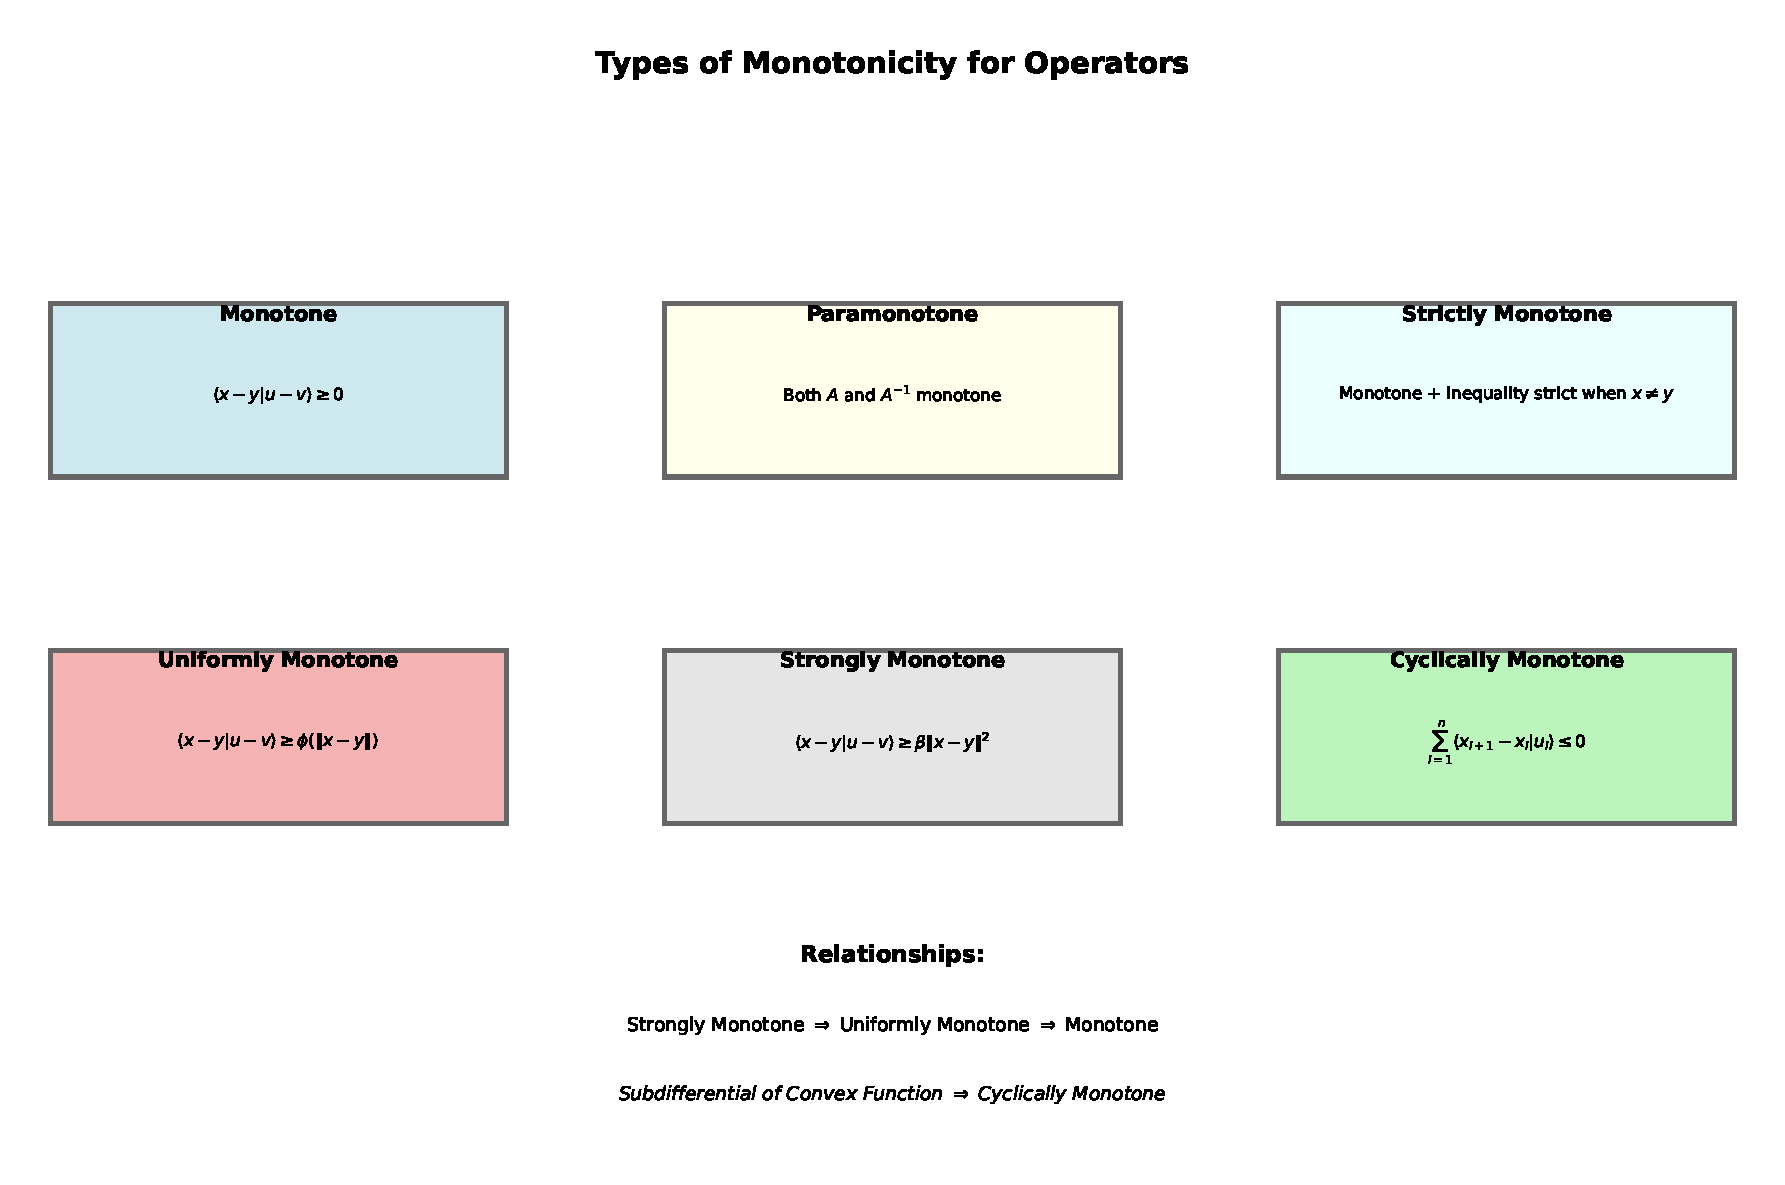
\includegraphics[width=\textwidth]{fig_monotonicity_types_detailed.pdf}
    \end{center}
\end{frame}

\begin{frame}{Key Relationships}
    \begin{tabular}{|c|c|c|}
        \hline
        \textbf{Property} & \textbf{Definition} & \textbf{Implication} \\
        \hline
        Monotone & $\langle x - y | u - v \rangle \geq 0$ & Basic concept \\
        \hline
        Paramonotone & $A$ and $A^{-1}$ both monotone & Invertibility preserved \\
        \hline
        Strictly Monotone & Monotone + strict when $x \neq y$ & Injectivity \\
        \hline
        Uniformly Monotone & $\langle x - y | u - v \rangle \geq \phi(\|x-y\|)$ & Rate control \\
        \hline
        Strongly Monotone & $\langle x - y | u - v \rangle \geq \beta\|x-y\|^2$ & Quadratic growth \\
        \hline
        Cyclically Monotone & $\sum_i \langle x_{i+1} - x_i | u_i \rangle \leq 0$ & Subdifferential \\
        \hline
    \end{tabular}

    \vspace{0.5cm}
    \begin{center}
        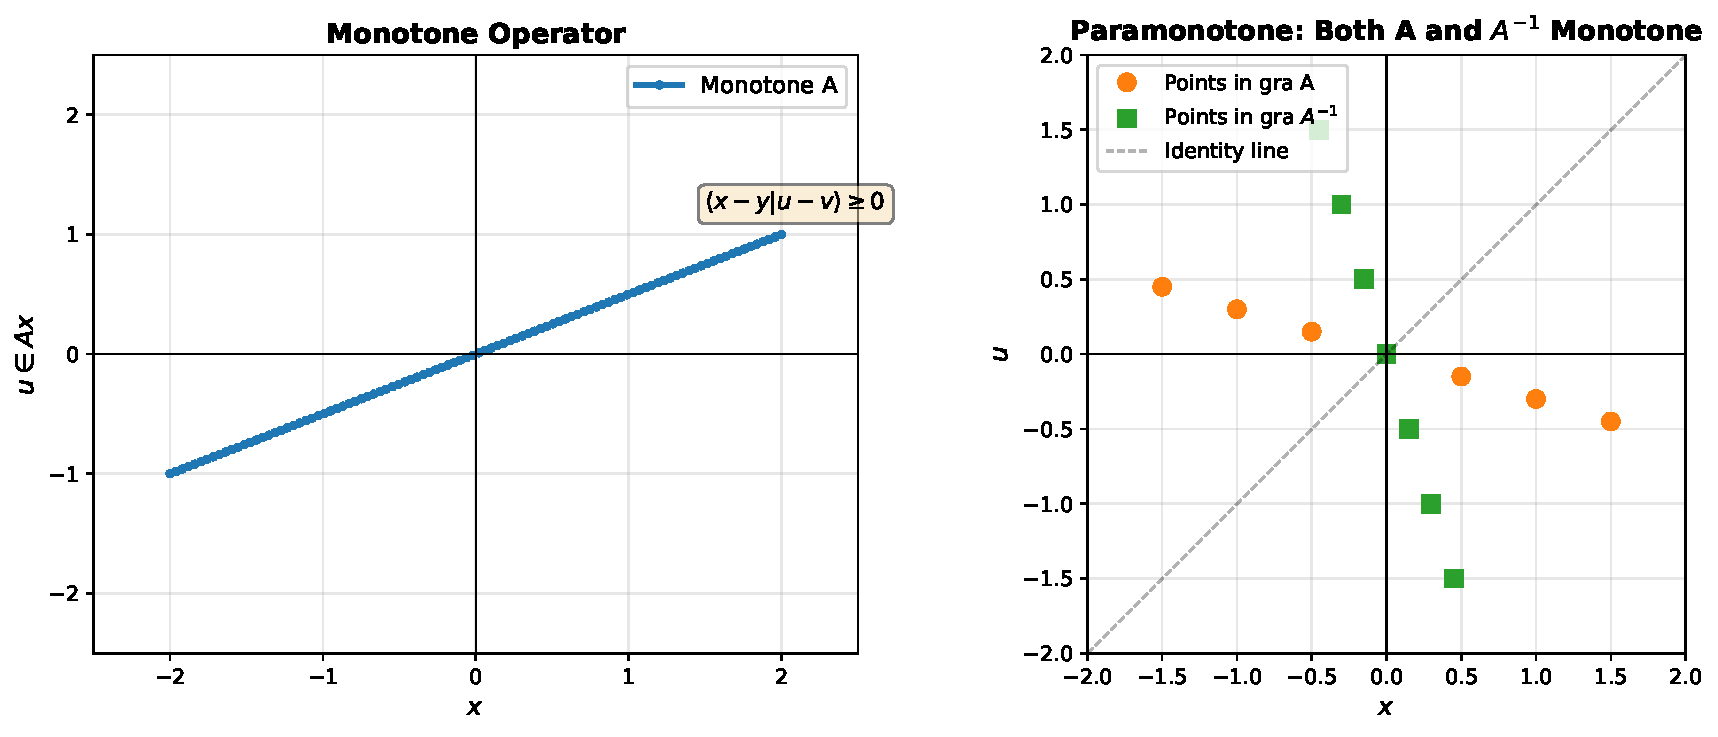
\includegraphics[width=0.7\textwidth]{fig_monotonicity_types.pdf}
    \end{center}
\end{frame}

\begin{frame}{Central Theorems}
    \begin{columns}
        \column{0.5\textwidth}
        \textbf{Subdifferentials are Cyclically Monotone:}

        If $f \in \Gamma_0(\mathcal{H})$, then
        $$\partial f \text{ is cyclically monotone}$$
        (Proposition 22.14)

        \vspace{0.5cm}
        \textbf{Uniqueness of Representation:}

        If $\partial f = \partial g$, then
        $$f = g + \gamma$$
        for some $\gamma \in \mathbb{R}$
        (Proposition 22.19)

        \column{0.5\textwidth}
        \textbf{Rockafellar's Theorem:}

        An operator $A$ is maximally cyclically monotone if and only if
        $$A = \partial f$$
        for some $f \in \Gamma_0(\mathcal{H})$
        (Theorem 22.18)

        \vspace{0.5cm}
        \textbf{One-Dimensional Case:}

        In $\mathbb{R}$, monotone $\Leftrightarrow$ cyclically monotone
        (Theorem 22.22)
    \end{columns}
\end{frame}

\begin{frame}{Numerical Examples and Visualizations}
    \begin{center}
        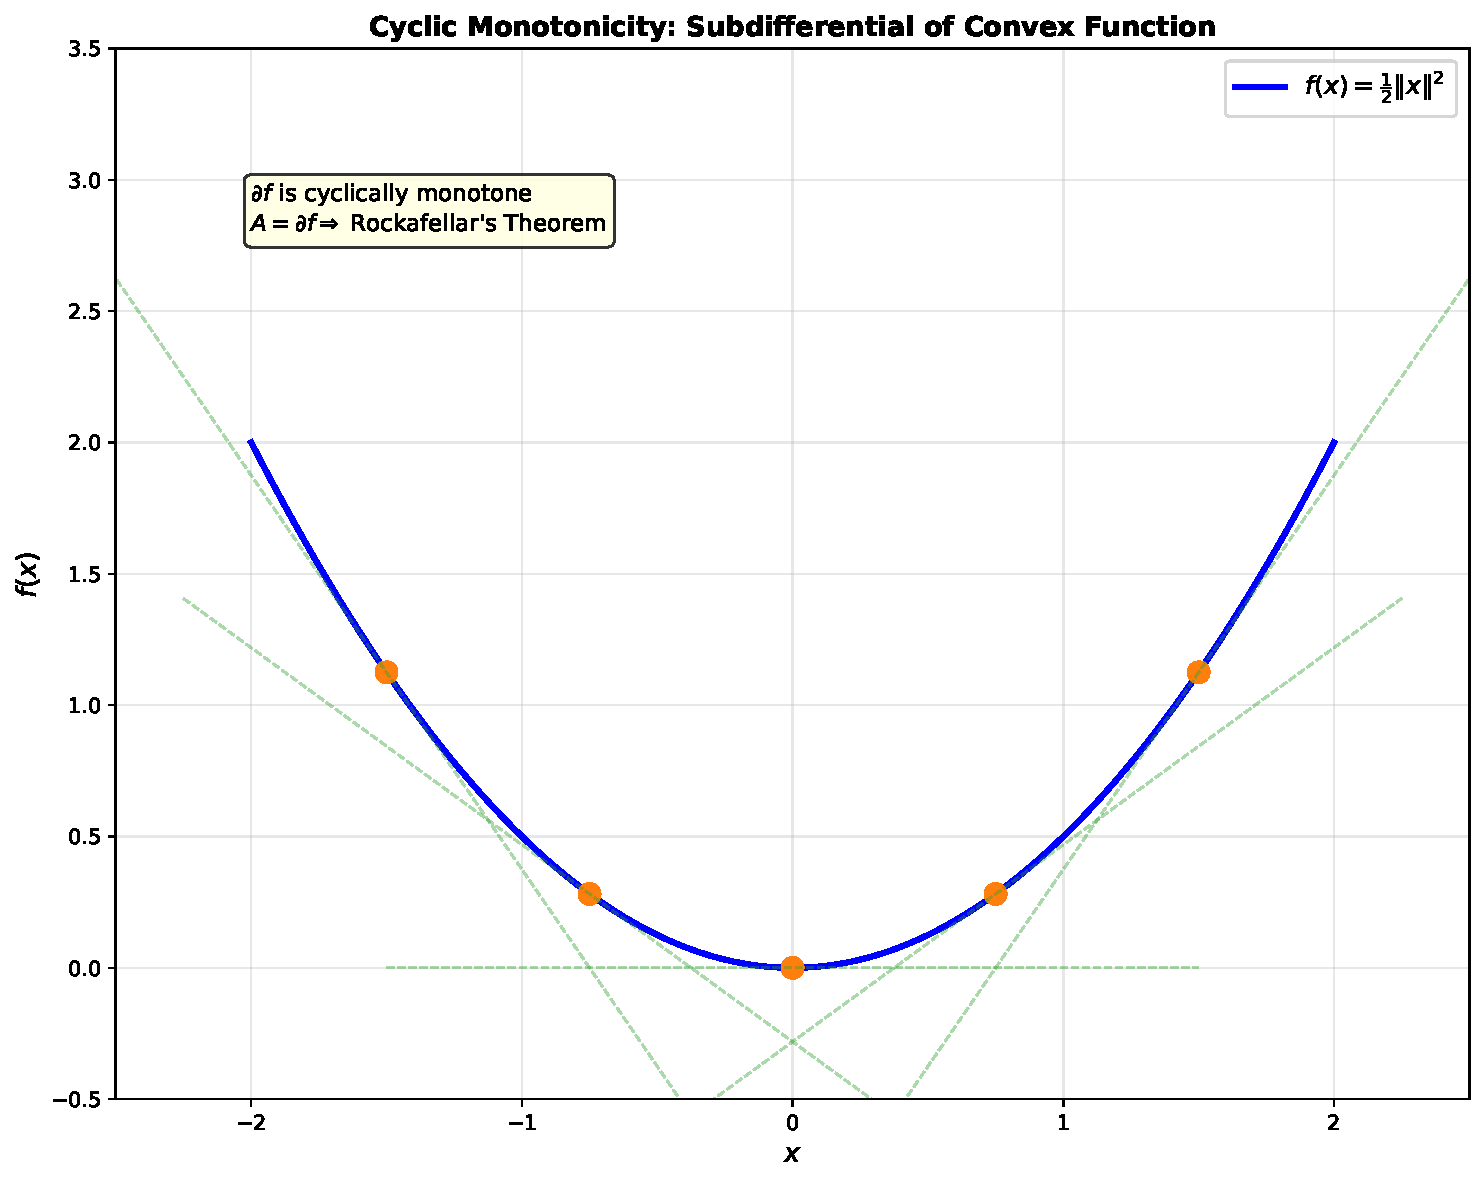
\includegraphics[width=0.8\textwidth]{fig_cyclic_monotonicity.pdf}
    \end{center}

    The subdifferential of $f(x) = \frac{1}{2}\|x\|^2$ is $\partial f(x) = \{x\}$
    (the gradient), which is cyclically monotone by Proposition 22.14.
\end{frame}

\begin{frame}[fragile]{Python: Testing Cyclic Monotonicity}
    \begin{lstlisting}[language=Python]
import numpy as np

def check_cyclic_monotone(graph, n=3):
    """Check if finite cycle satisfies cyclic monotonicity"""
    points = list(graph)
    if len(points) < n:
        return None

    # Test n-cyclic monotonicity
    for i in range(len(points) - n + 1):
        x_vals = [p[0] for p in points[i:i+n]]
        u_vals = [p[1] for p in points[i:i+n]]

        # Compute sum of inner products
        cyclic_sum = 0
        for j in range(n):
            dx = x_vals[(j+1) % n] - x_vals[j]
            cyclic_sum += np.dot(dx, u_vals[j])

        if cyclic_sum > 1e-10:  # tolerance
            return False

    return True

# Example: subdifferential of f(x) = (1/2)||x||^2
# which is partial_f(x) = {x}
graph = [
    (np.array([-1.0, -1.0]), np.array([-1.0, -1.0])),
    (np.array([0.0, 1.0]), np.array([0.0, 1.0])),
    (np.array([1.0, 0.0]), np.array([1.0, 0.0]))
]

result = check_cyclic_monotone(graph, n=3)
print(f"Cyclically monotone: {result}")  # True
    \end{lstlisting}
\end{frame}

\begin{frame}[fragile]{Python: Verifying Operator Properties}
    \begin{lstlisting}[language=Python]
import numpy as np

def is_monotone(x1, u1, x2, u2):
    """Check monotonicity: <x1-x2 | u1-u2> >= 0"""
    dx = x1 - x2
    du = u1 - u2
    return np.dot(dx, du) >= -1e-10  # tolerance

def is_strongly_monotone(x1, u1, x2, u2, beta):
    """Check strong monotonicity: <x-y|u-v> >= beta||x-y||^2"""
    dx = x1 - x2
    du = u1 - u2
    return np.dot(dx, du) >= beta * np.dot(dx, dx) - 1e-10

# Example: A(x) = x (identity - strongly monotone with beta=1)
x1 = np.array([2.0, 1.0])
x2 = np.array([1.0, 3.0])
u1 = x1  # A(x1) = x1
u2 = x2  # A(x2) = x2

print(f"Monotone: {is_monotone(x1, u1, x2, u2)}")  # True
print(f"Strongly monotone (beta=1): {is_strongly_monotone(x1, u1, x2, u2, 1.0)}")  # True
print(f"Strongly monotone (beta=2): {is_strongly_monotone(x1, u1, x2, u2, 2.0)}")  # False

# Verification
dx = x1 - x2
du = u1 - u2
inner = np.dot(dx, du)
print(f"<x1-x2|u1-u2> = {inner}, ||x1-x2||^2 = {np.dot(dx,dx)}")
    \end{lstlisting}
\end{frame}

\begin{frame}{Example Computations}
    \begin{example}
        Let $\mathcal{H} = \mathbb{R}^2$ and $f(x) = \frac{1}{2}\|x\|^2$.

        \textbf{Claim:} $\partial f$ is strongly monotone with constant $\beta = 1$.

        \textbf{Verification:}
        \begin{itemize}
            \item For all $x, y \in \mathbb{R}^2$: $\partial f(x) = \{x\}$
            \item Take $(x, u) = (x, x)$ and $(y, v) = (y, y)$ in $\text{gra}(\partial f)$
            \item Then:
                \begin{align}
                    \langle x - y | u - v \rangle &= \langle x - y | x - y \rangle \\
                    &= \|x - y\|^2 \geq 1 \cdot \|x - y\|^2
                \end{align}
            \item So $\partial f$ is strongly monotone with $\beta = 1$.
        \end{itemize}
    \end{example}
\end{frame}

\begin{frame}{Applications to Optimization}
    \begin{itemize}
        \item \textbf{Existence and Uniqueness:} Strong monotonicity of $\partial f$ implies
              the equation $\partial f(x) \ni r$ has a unique solution.

        \item \textbf{Algorithm Design:} Monotonicity properties guide the design of
              splitting methods (gradient descent, proximal methods, ADMM, etc.).

        \item \textbf{Convergence Analysis:} Different monotonicity constants determine
              convergence rates of algorithms.

        \item \textbf{Structure Preservation:} Paramonotonicity ensures that compositions
              and combinations of operators retain nice properties.

        \item \textbf{Inverse Problems:} Monotone operators are fundamental in
              regularization and ill-posed problem solving.
    \end{itemize}
\end{frame}

\begin{frame}{Further Visualization}
    \begin{center}
        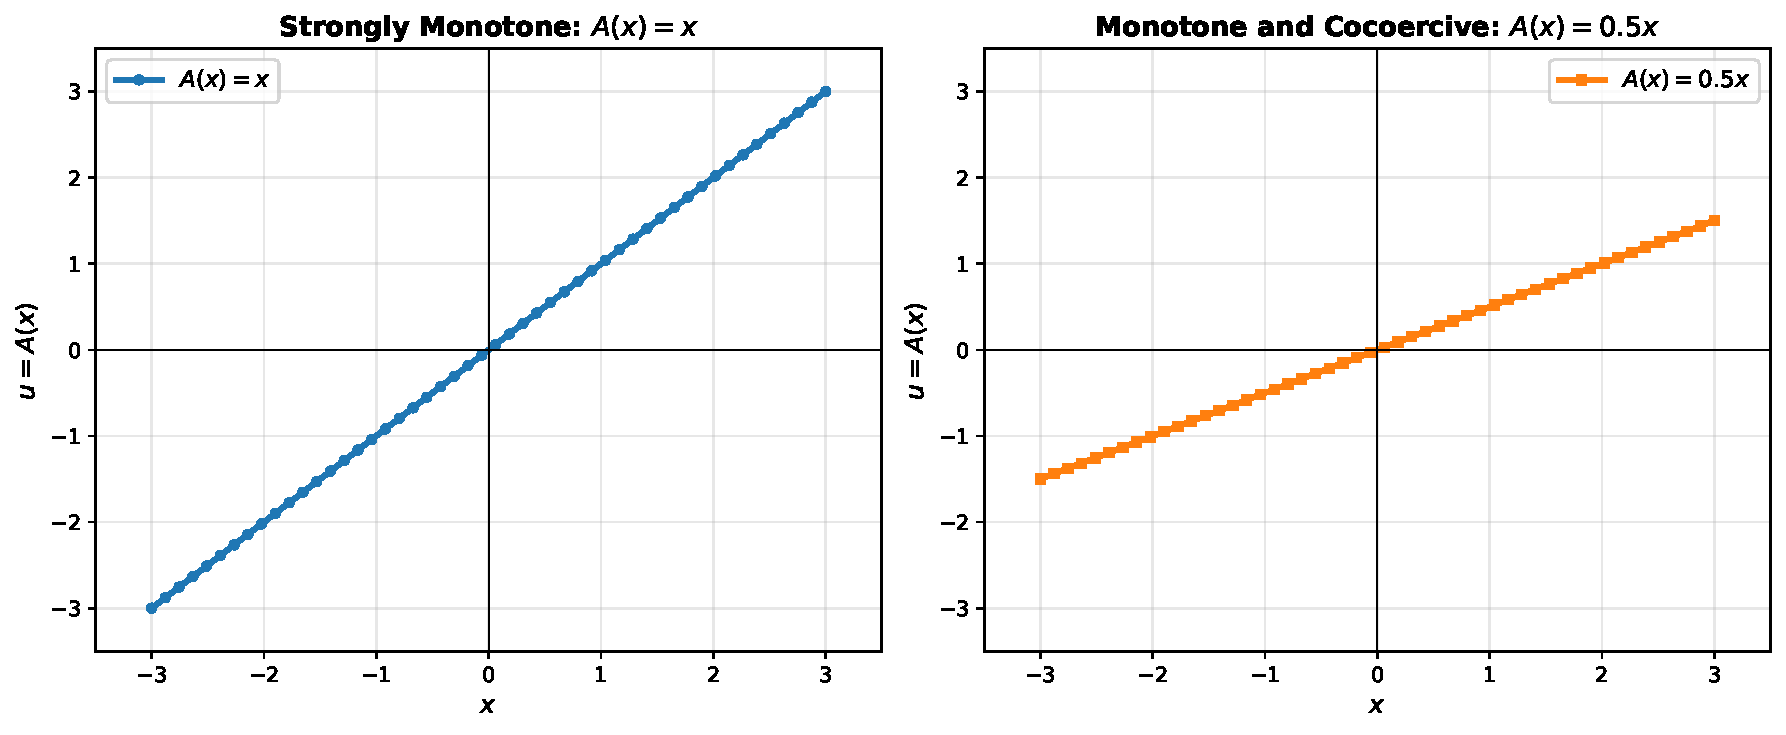
\includegraphics[width=0.8\textwidth]{fig_monotone_examples.pdf}
    \end{center}

    Examples of monotone operators: the identity $A(x) = x$ (strongly monotone)
    and the scaled identity $A(x) = 0.5x$ (monotone and cocoercive).
\end{frame}

\begin{frame}{Key Takeaways}
    \begin{enumerate}
        \item \textbf{Multiple notions of monotonicity} exist, ranging from basic to strongly structured:
            paramonotone, strictly, uniformly, and strongly monotone.

        \item \textbf{Cyclic monotonicity} is a fundamental concept that characterizes subdifferentials
              of proper convex functions via Rockafellar's theorem.

        \item \textbf{Rockafellar's Theorem} (22.18) provides a complete characterization:
              An operator is maximally cyclically monotone $\Leftrightarrow$ it is a subdifferential.

        \item \textbf{Subdifferentials are always cyclically monotone} (Proposition 22.14),
              while not all monotone operators are cyclically monotone (Example 22.15).

        \item \textbf{In one dimension}, monotone and cyclically monotone are equivalent
              (Theorem 22.22), making the structure much simpler.

        \item These concepts are \textbf{essential for optimization algorithms} and
              inverse problem analysis.
    \end{enumerate}
\end{frame}

\begin{frame}{References and Further Study}
    \begin{itemize}
        \item \textbf{Primary Reference:} Bauschke, H.H., and Combettes, P.L.
              \emph{Convex Analysis and Monotone Operator Theory in Hilbert Spaces}.
              Springer, 2017. Chapter 22.

        \item \textbf{Key Theorems:}
            \begin{itemize}
                \item Proposition 22.2: Paramonotonicity preservation
                \item Proposition 22.14: Subdifferentials are cyclically monotone
                \item Theorem 22.18 (Rockafellar): Cyclic monotonicity characterization
                \item Theorem 22.22: One-dimensional equivalence
            \end{itemize}

        \item \textbf{Related Chapters:} Chapter 20 (Monotone Operators),
              Chapter 21 (Comonotonicity), Chapter 23 (Resolvents).

        \item \textbf{Applications:} Convex optimization, variational inequalities,
              splitting methods, proximal algorithms.
    \end{itemize}
\end{frame}

\end{document}
